\section{Price response functions}
\label{sec:response_functions}
In Sect. \ref{subsec:key_concepts} we establish the fundamental quantities used
in the price response definitions.
In Sect. \ref{subsec:response_function_trade} we analyze the responses
functions in trade time scale and in Sect. \ref{subsec:response_function_physical}
we analyze the responses functions in physical time scale.

%%%%%%%%%%%%%%%%%%%%%%%%%%%%%%%%%%%%%%%%%%%%%%%%%%%%%%%%%%%%%%%%%%%%%%%%%%%%%%%
\subsection{Key concepts}\label{subsec:key_concepts}

In general, three categories of currency pairs are defined: majors, crosses,
and exotics. The ``major'' foreign exchange currency pairs are the major
countries that are paired with the U.S. dollar (see Table \ref{tab:majors}).
The ``crosses'' are those majors pairs that are not paired against the U.S.
dollar. Finally, the ``exotic'' pairs usually consist of a major currency
alongside a thinly traded currency or an emerging market economy currency.
The majors are the most liquid pairs, in contrast with the exotics, who can be
much more volatile.

In foreign exchange markets, orders are execute at the best available buy or
sell price. Orders often fail to result in an immediate transaction, and are
stored in a queue called the limit order book
\cite{stat_prop,predictive_pow,forex_structure,intro_market_micro,forex_market_micro,prop_order_book}.
The order book is visible for all traders and its main purpose is to ensure
that all traders have the same information on what is offered on the market.
For a detailed description of the operation of the markets, we suggest to see
Ref. \cite{my_paper_response_financial}.

At any given time there is a best (lowest) offer to sell with price
$a\left(t\right)$, and a best (highest) bid to buy with price $b\left(t\right)$
\cite{subtle_nature,account_spread,limit_ord_spread,prop_order_book,stat_theory}.
The price gap between them is called the spread
$s\left(t\right) = a\left(t\right)-b\left(t\right)$
\cite{subtle_nature,market_digest,Bouchaud_2004,account_spread,teach_spread,large_prices_changes,em_stylized_facts,stat_theory}.
Spreads are significantly positively related to price and significantly
negatively related to trading volume. Companies with more liquidity tend to
have lower spreads
\cite{components_spread_tokyo,effects_spread,account_spread,components_spread}.
Despite the foreign exchange market is often cited as the world's largest
financial market, this description fail to consider the considerable differences
in trading volume and liquidity across different currency pairs
\cite{forex_microstructure}. These differences can be directly seen in the
spread. Furthermore, the bid-ask spread is directly related with the
transaction costs to the dealer \cite{teach_spread,spread_futures}.

Due to the lack of prices information in the data, we consider a basic
definition of the price given by
\cite{patterns_forex,political_forex,forex_liquidity}. The average of the best
ask and the best bid is the midpoint price, which is defined as
\cite{subtle_nature,Bouchaud_2004,teach_spread,large_prices_changes,my_paper_response_financial,em_stylized_facts,prop_order_book,stat_theory}

\begin{equation}
    m \left(t\right) = \frac{a\left(t\right) + b\left(t\right)}{2}
\end{equation}

Price changes are typically characterized as returns. If one denotes
$S\left( t\right)$ the price of an asset at time $t$, the return
$r\left(t, \tau\right)$, at time $t$ and time lag $\tau$ is simply the relative
variation of the price from $t$ to $t + \tau$
\cite{subtle_nature,empirical_facts,asynchrony_effects_corr,tick_size_impact,causes_epps_effect,non_stationarity},
\begin{equation}\label{eq:return_general}
    r^{\left(g\right)} \left(t, \tau \right) = \frac{S\left(t + \tau\right)
    - S\left(t\right)}{S\left(t\right)}
\end{equation}

We define the returns via the midpoint price as
\begin{equation}\label{eq:midpoint_price_return}
    r\left(t,\tau\right) = \frac{m\left(t+\tau\right)-m\left(t\right)}
    {m\left(t\right)}
\end{equation}
The distribution of returns is strongly non-Gaussian and its shape continuously
depends on the return period $\tau$. Small $\tau$ values have fat tails return
distributions \cite{subtle_nature}. The trade signs are defined for general
cases as
\begin{equation}\label{eq:trade_sign_general}
    \varepsilon\left(t\right)=\text{sign}\left(S\left(t\right)
    -m\left(t-\delta\right)\right)
\end{equation}
where $\delta$ is a positive time increment. Hence we have
\begin{equation}\label{eq:trade_sign_results}
    \varepsilon\left(t\right)=\left\{
    \begin{array}{cc}
    +1, & \text{If } S\left(t\right)
    \text{ is higher than the last } m\left( t \right)\\
    -1, & \text{If } S\left(t\right)
    \text{ is lower than the last } m\left( t \right)
    \end{array}\right.
\end{equation}
$\varepsilon(t) = +1$ indicates that the trade was triggered by a market order
to buy and a trade triggered by a market order to sell yields
$\varepsilon(t) = -1$
\cite{subtle_nature,Bouchaud_2004,spread_changes_affect,quant_stock_price_response,order_flow_persistent}.

The main objective of this work is to analyze the price response functions. In
general we define the price response functions in a foreign exchange market as
\begin{equation}\label{eq:response_general}
    R^{\left(scale\right)}_{ii}\left(\tau\right)=\left\langle
    r^{\left(scale\right)}_{i}\left(t-1, \tau\right)
    \varepsilon^{\left(scale\right)}_{i} \left(t\right)\right\rangle_{average}
\end{equation}
where the index $i$ correspond to currency pairs in the market,
$r^{\left(scale\right)}_{i}$ is the return of the pair $i$ in a time lag $\tau$
in the corresponding scale and $\varepsilon^{\left(scale\right)}_{i}$ is the
trade sign of the pair $i$ in the corresponding scale. The superscript $scale$
refers to the time scale used, whether physical time scale
($scale = p$) or trade time scale ($scale = t$). Finally, The subscript
$average$ refers to the way to average the price response, whether relative to
the physical time scale ($average = P$) or relative to the trade time scale
($average = T$).

%%%%%%%%%%%%%%%%%%%%%%%%%%%%%%%%%%%%%%%%%%%%%%%%%%%%%%%%%%%%%%%%%%%%%%%%%%%%%%%
\subsection{Response functions on trade time scale}
\label{subsec:response_function_trade}

The price response function in trade time scale is defined as
\begin{equation}\label{eq:response_functions_trade_scale_general}
    R^{\left(t\right)}_{ii}\left(\tau\right)=\left\langle r^{\left(p\right)}
    _{i}\left(t-1,\tau \right)\varepsilon_{i}^{\left(t\right)}
    \left(t, n\right)\right\rangle _{T}
\end{equation}
where the superscript $t$ refers to the trade time scale.

To compute the response functions on trade time scale, we used all the trade
signs during a week in market time.

\begin{figure}[htbp]
    \centering
    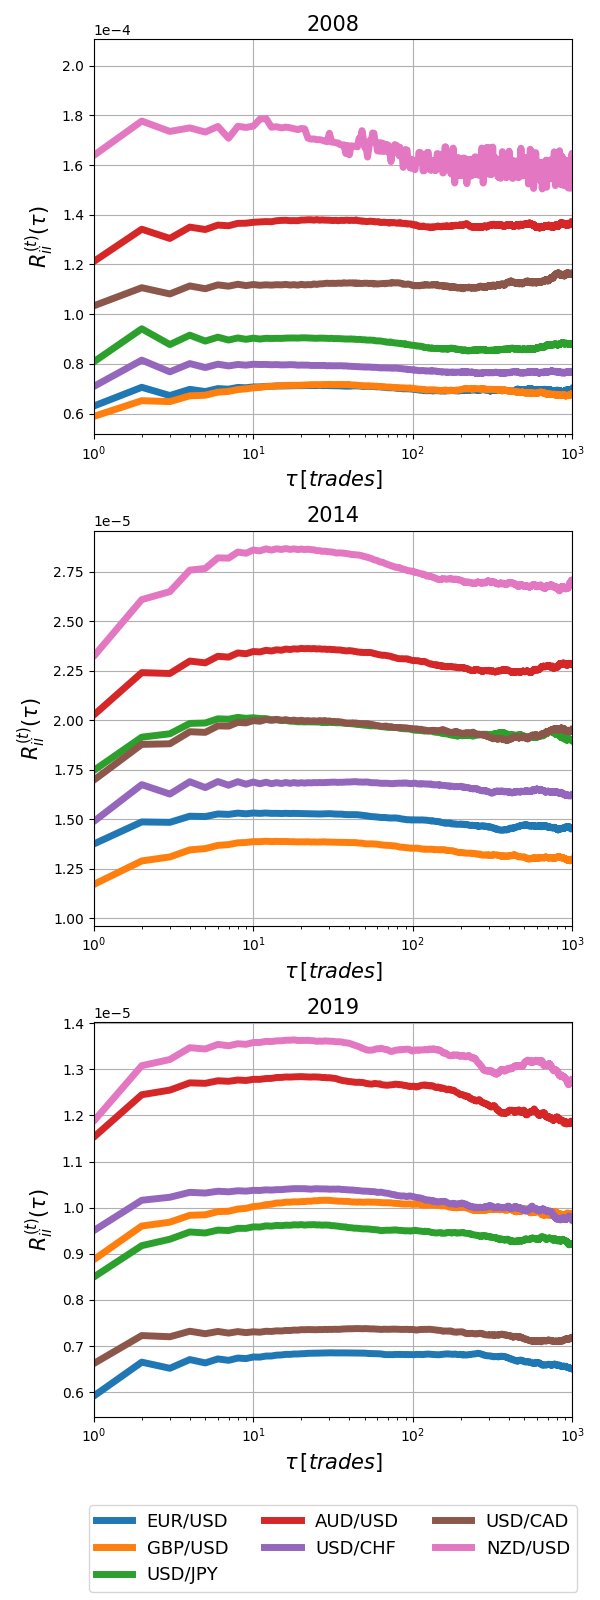
\includegraphics[width=\columnwidth]
    {figures/04_responses_trade_scale.png}
    \caption{Price response functions
             $R^{\left(t\right)}_{ij}\left(\tau\right)$ versus time lag $\tau$
             on a logarithmic scale in trade time scale for the years 2008
             (top), 2014 (middle) and 2019 (bottom).}
    \label{fig:response_function_trade_scale}
\end{figure}

% The results of Fig. \ref{fig:response_function_trade_scale} show the self-
% responses of the six stocks used in the analysis and the cross-responses for
% pairs of stocks representing three different economic sectors.

% The self-response functions increase to a maximum and then slowly decrease. In
% some stocks this behavior is more pronounced than in others. For our selected
% tickers, a time lag of $\tau = 10^{3}s$ is enough to see an increase to a
% maximum followed by a decrease. Thus, the trend in the self-response functions
% is eventually reversed.
% On the other hand, the cross-response functions have smaller signal strength
% than the self-response functions. For our cross-response functions of stocks in
% the same sectors, some couples exhibit the increase-decrease behavior inside a
% time lag of $\tau = 10^{3}s$. Other couples seems to need a larger time lag to
% reach the decrease behavior.

%%%%%%%%%%%%%%%%%%%%%%%%%%%%%%%%%%%%%%%%%%%%%%%%%%%%%%%%%%%%%%%%%%%%%%%%%%%%%%%
\subsection{Response functions on physical time scale}
\label{subsec:response_function_physical}

One important detail to compute the market response in physical time scale is
to define how the averaging of the function will be made, because the
response functions highly differ when we include or exclude
$\varepsilon^{\left(p\right)}_j \left( t\right) = 0$ \cite{Wang_2016_cross}.
The cross-responses including
$\varepsilon^{\left(p\right)}_j \left( t\right) = 0$ are weaker than the
excluding ones due to the omission of direct influence of the lack of trades.
However, either including or excluding $\varepsilon^{p}_j \left( t\right) = 0$
does not change the trend of price reversion versus the time lag, but it does
affect the response function strength \cite{Wang_2016_avg}. For a deeper
analysis of the influence of the term
$\varepsilon^{\left(p\right)}_j \left( t\right) = 0$, we suggest to check Refs.
\cite{Wang_2016_avg,Wang_2016_cross}. We will only take in account the
cross-response function excluding $\varepsilon^{p}_j \left( t\right) = 0$.

We define the price response functions in physical time scale, using
the trade signs and the returns in physical time scale. The price response
function on physical time scale is defined as
\begin{equation}\label{eq:response_functions_time_scale_general}
    R^{\left(p\right)}_{ii}\left(\tau\right)=\left\langle r^{\left(p\right)}
    _{i}\left(t-1, \tau\right) \varepsilon_{i}^{\left(p\right)} \left(t\right)
    \right\rangle _{P}
\end{equation}
where the superscript $p$ refers to the physical time scale.

\begin{figure}[htbp]
    \centering
    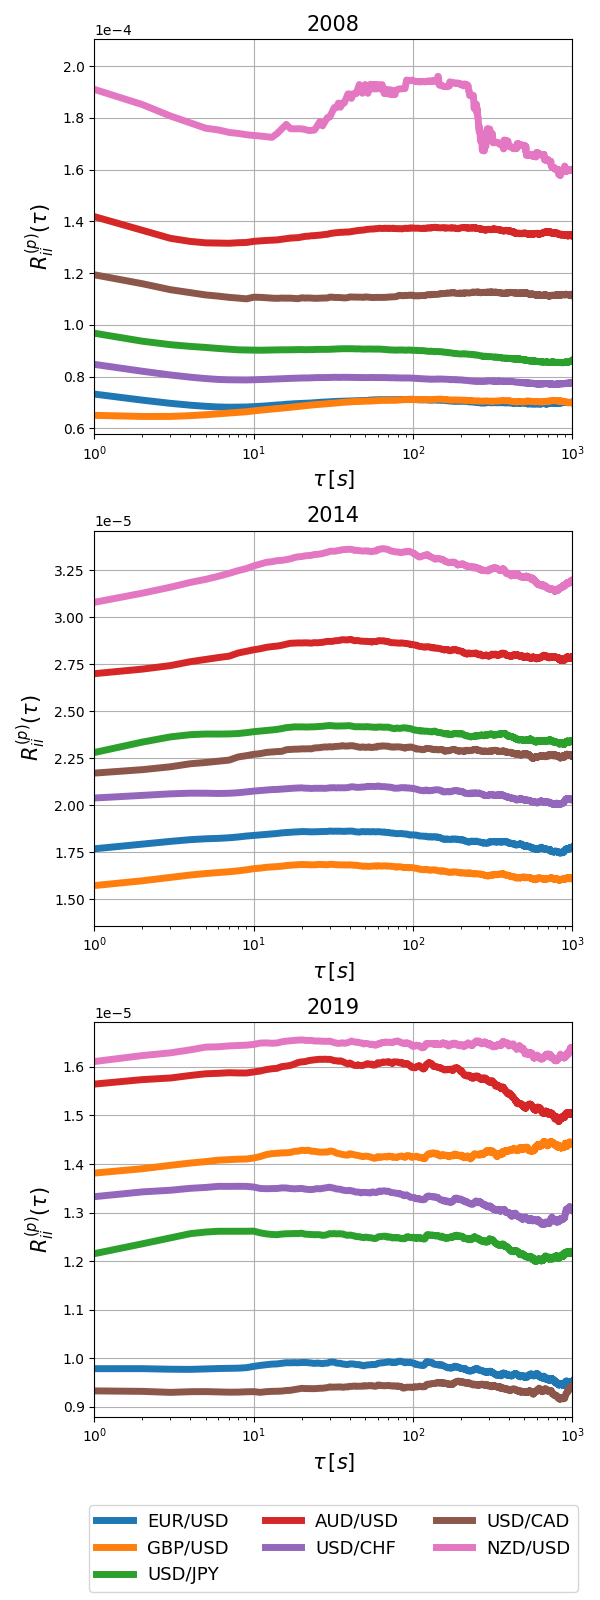
\includegraphics[width=\columnwidth]
    {figures/04_responses_physical_scale.png}
    \caption{Price response functions
             $R^{\left(p\right)}_{ij}\left(\tau\right)$ excluding
             $\varepsilon^{\left(p\right)}_{i}\left(t\right) = 0$ versus time
             lag $\tau$ on a logarithmic scale in physical time scale for the
             years 2008 (top), 2014 (middle) and 2019 (bottom).}
    \label{fig:market_response_time_scale}
\end{figure}

% The results showed in Fig. \ref{fig:market_response_time_scale} are the
% self- and cross-response functions in physical time scale. For the
% self-response functions we can say again that in almost all the cases, an
% increase to a maximum is followed by a decrease. Thus, the trend in the self-
% and cross-response is eventually reversed.
% In the cross-response functions, we have a similar behavior with the previous
% subsection, where the time lag in some pairs was not enough to see the decrease
% of the response.

% Compared with the response functions in trade time scale, the response functions
% in physical time scale are stronger.